% Options for packages loaded elsewhere
% Options for packages loaded elsewhere
\PassOptionsToPackage{unicode}{hyperref}
\PassOptionsToPackage{hyphens}{url}
\PassOptionsToPackage{dvipsnames,svgnames,x11names}{xcolor}
%
\documentclass[
  ngerman,
  letterpaper,
  DIV=11]{scrreprt}
\usepackage{xcolor}
\usepackage{amsmath,amssymb}
\setcounter{secnumdepth}{2}
\usepackage{iftex}
\ifPDFTeX
  \usepackage[T1]{fontenc}
  \usepackage[utf8]{inputenc}
  \usepackage{textcomp} % provide euro and other symbols
\else % if luatex or xetex
  \usepackage{unicode-math} % this also loads fontspec
  \defaultfontfeatures{Scale=MatchLowercase}
  \defaultfontfeatures[\rmfamily]{Ligatures=TeX,Scale=1}
\fi
\usepackage{lmodern}
\ifPDFTeX\else
  % xetex/luatex font selection
\fi
% Use upquote if available, for straight quotes in verbatim environments
\IfFileExists{upquote.sty}{\usepackage{upquote}}{}
\IfFileExists{microtype.sty}{% use microtype if available
  \usepackage[]{microtype}
  \UseMicrotypeSet[protrusion]{basicmath} % disable protrusion for tt fonts
}{}
\makeatletter
\@ifundefined{KOMAClassName}{% if non-KOMA class
  \IfFileExists{parskip.sty}{%
    \usepackage{parskip}
  }{% else
    \setlength{\parindent}{0pt}
    \setlength{\parskip}{6pt plus 2pt minus 1pt}}
}{% if KOMA class
  \KOMAoptions{parskip=half}}
\makeatother
% Make \paragraph and \subparagraph free-standing
\makeatletter
\ifx\paragraph\undefined\else
  \let\oldparagraph\paragraph
  \renewcommand{\paragraph}{
    \@ifstar
      \xxxParagraphStar
      \xxxParagraphNoStar
  }
  \newcommand{\xxxParagraphStar}[1]{\oldparagraph*{#1}\mbox{}}
  \newcommand{\xxxParagraphNoStar}[1]{\oldparagraph{#1}\mbox{}}
\fi
\ifx\subparagraph\undefined\else
  \let\oldsubparagraph\subparagraph
  \renewcommand{\subparagraph}{
    \@ifstar
      \xxxSubParagraphStar
      \xxxSubParagraphNoStar
  }
  \newcommand{\xxxSubParagraphStar}[1]{\oldsubparagraph*{#1}\mbox{}}
  \newcommand{\xxxSubParagraphNoStar}[1]{\oldsubparagraph{#1}\mbox{}}
\fi
\makeatother


\usepackage{longtable,booktabs,array}
\usepackage{calc} % for calculating minipage widths
% Correct order of tables after \paragraph or \subparagraph
\usepackage{etoolbox}
\makeatletter
\patchcmd\longtable{\par}{\if@noskipsec\mbox{}\fi\par}{}{}
\makeatother
% Allow footnotes in longtable head/foot
\IfFileExists{footnotehyper.sty}{\usepackage{footnotehyper}}{\usepackage{footnote}}
\makesavenoteenv{longtable}
\usepackage{graphicx}
\makeatletter
\newsavebox\pandoc@box
\newcommand*\pandocbounded[1]{% scales image to fit in text height/width
  \sbox\pandoc@box{#1}%
  \Gscale@div\@tempa{\textheight}{\dimexpr\ht\pandoc@box+\dp\pandoc@box\relax}%
  \Gscale@div\@tempb{\linewidth}{\wd\pandoc@box}%
  \ifdim\@tempb\p@<\@tempa\p@\let\@tempa\@tempb\fi% select the smaller of both
  \ifdim\@tempa\p@<\p@\scalebox{\@tempa}{\usebox\pandoc@box}%
  \else\usebox{\pandoc@box}%
  \fi%
}
% Set default figure placement to htbp
\def\fps@figure{htbp}
\makeatother

\ifLuaTeX
  \usepackage{luacolor}
  \usepackage[soul]{lua-ul}
\else
  \usepackage{soul}
\fi

% definitions for citeproc citations
\NewDocumentCommand\citeproctext{}{}
\NewDocumentCommand\citeproc{mm}{%
  \begingroup\def\citeproctext{#2}\cite{#1}\endgroup}
\makeatletter
 % allow citations to break across lines
 \let\@cite@ofmt\@firstofone
 % avoid brackets around text for \cite:
 \def\@biblabel#1{}
 \def\@cite#1#2{{#1\if@tempswa , #2\fi}}
\makeatother
\newlength{\cslhangindent}
\setlength{\cslhangindent}{1.5em}
\newlength{\csllabelwidth}
\setlength{\csllabelwidth}{3em}
\newenvironment{CSLReferences}[2] % #1 hanging-indent, #2 entry-spacing
 {\begin{list}{}{%
  \setlength{\itemindent}{0pt}
  \setlength{\leftmargin}{0pt}
  \setlength{\parsep}{0pt}
  % turn on hanging indent if param 1 is 1
  \ifodd #1
   \setlength{\leftmargin}{\cslhangindent}
   \setlength{\itemindent}{-1\cslhangindent}
  \fi
  % set entry spacing
  \setlength{\itemsep}{#2\baselineskip}}}
 {\end{list}}
\usepackage{calc}
\newcommand{\CSLBlock}[1]{\hfill\break\parbox[t]{\linewidth}{\strut\ignorespaces#1\strut}}
\newcommand{\CSLLeftMargin}[1]{\parbox[t]{\csllabelwidth}{\strut#1\strut}}
\newcommand{\CSLRightInline}[1]{\parbox[t]{\linewidth - \csllabelwidth}{\strut#1\strut}}
\newcommand{\CSLIndent}[1]{\hspace{\cslhangindent}#1}

\ifLuaTeX
\usepackage[bidi=basic]{babel}
\else
\usepackage[bidi=default]{babel}
\fi
% get rid of language-specific shorthands (see #6817):
\let\LanguageShortHands\languageshorthands
\def\languageshorthands#1{}
\ifLuaTeX
  \usepackage[german]{selnolig} % disable illegal ligatures
\fi


\setlength{\emergencystretch}{3em} % prevent overfull lines

\providecommand{\tightlist}{%
  \setlength{\itemsep}{0pt}\setlength{\parskip}{0pt}}



 


\KOMAoption{captions}{tableheading}
\makeatletter
\@ifpackageloaded{tcolorbox}{}{\usepackage[skins,breakable]{tcolorbox}}
\@ifpackageloaded{fontawesome5}{}{\usepackage{fontawesome5}}
\definecolor{quarto-callout-color}{HTML}{909090}
\definecolor{quarto-callout-note-color}{HTML}{0758E5}
\definecolor{quarto-callout-important-color}{HTML}{CC1914}
\definecolor{quarto-callout-warning-color}{HTML}{EB9113}
\definecolor{quarto-callout-tip-color}{HTML}{00A047}
\definecolor{quarto-callout-caution-color}{HTML}{FC5300}
\definecolor{quarto-callout-color-frame}{HTML}{acacac}
\definecolor{quarto-callout-note-color-frame}{HTML}{4582ec}
\definecolor{quarto-callout-important-color-frame}{HTML}{d9534f}
\definecolor{quarto-callout-warning-color-frame}{HTML}{f0ad4e}
\definecolor{quarto-callout-tip-color-frame}{HTML}{02b875}
\definecolor{quarto-callout-caution-color-frame}{HTML}{fd7e14}
\makeatother
\makeatletter
\@ifpackageloaded{bookmark}{}{\usepackage{bookmark}}
\makeatother
\makeatletter
\@ifpackageloaded{caption}{}{\usepackage{caption}}
\AtBeginDocument{%
\ifdefined\contentsname
  \renewcommand*\contentsname{Inhaltsverzeichnis}
\else
  \newcommand\contentsname{Inhaltsverzeichnis}
\fi
\ifdefined\listfigurename
  \renewcommand*\listfigurename{Abbildungsverzeichnis}
\else
  \newcommand\listfigurename{Abbildungsverzeichnis}
\fi
\ifdefined\listtablename
  \renewcommand*\listtablename{Tabellenverzeichnis}
\else
  \newcommand\listtablename{Tabellenverzeichnis}
\fi
\ifdefined\figurename
  \renewcommand*\figurename{Abbildung}
\else
  \newcommand\figurename{Abbildung}
\fi
\ifdefined\tablename
  \renewcommand*\tablename{Tabelle}
\else
  \newcommand\tablename{Tabelle}
\fi
}
\@ifpackageloaded{float}{}{\usepackage{float}}
\floatstyle{ruled}
\@ifundefined{c@chapter}{\newfloat{codelisting}{h}{lop}}{\newfloat{codelisting}{h}{lop}[chapter]}
\floatname{codelisting}{Listing}
\newcommand*\listoflistings{\listof{codelisting}{Listingverzeichnis}}
\makeatother
\makeatletter
\makeatother
\makeatletter
\@ifpackageloaded{caption}{}{\usepackage{caption}}
\@ifpackageloaded{subcaption}{}{\usepackage{subcaption}}
\makeatother
\usepackage{bookmark}
\IfFileExists{xurl.sty}{\usepackage{xurl}}{} % add URL line breaks if available
\urlstyle{same}
\hypersetup{
  pdftitle={KI als Hilfe zum Lehren und Lernen},
  pdfauthor={Roman Bartnik},
  pdflang={de},
  colorlinks=true,
  linkcolor={blue},
  filecolor={Maroon},
  citecolor={Blue},
  urlcolor={Blue},
  pdfcreator={LaTeX via pandoc}}


\title{KI als Hilfe zum Lehren und Lernen}
\author{Roman Bartnik}
\date{2025-12-05}
\begin{document}
\maketitle

\renewcommand*\contentsname{Inhaltsverzeichnis}
{
\hypersetup{linkcolor=}
\setcounter{tocdepth}{2}
\tableofcontents
}

\bookmarksetup{startatroot}

\chapter*{Übersicht}\label{uxfcbersicht}
\addcontentsline{toc}{chapter}{Übersicht}

\markboth{Übersicht}{Übersicht}

Dieses Buch untersucht, wie generative künstliche Intelligenz (GenAI)
Lehre, Lernen und Forschung verändern kann. Es richtet sich an Lehrende,
Forschende und Studierende, die verstehen möchten, \textbf{wie KI als
Werkzeug der Hochschuldidaktik} eingesetzt werden kann.

Das Buch besteht aus fünf Kapiteln:

\begin{enumerate}
\def\labelenumi{\arabic{enumi}.}
\tightlist
\item
  Überblick: KI als Hilfe zum Lehren und Lernen\\
\item
  Grundbegriffe und technische Grundlagen\\
\item
  Didaktische Prinzipien und Cognitive Science\\
\item
  Praxisbeispiele: KI als Hiwi, Copilot, Tutor, Simulator\\
\item
  Empfehlungen zur Umsetzung\\
\end{enumerate}

Im ersten Teil fassen wir die aktuelle Forschungslage zusammen.

\bookmarksetup{startatroot}

\chapter{Einleitung}\label{einleitung}

\section{KI als Hilfe für die
Lehre}\label{ki-als-hilfe-fuxfcr-die-lehre}

\textbf{Wie kann uns generative künstliche Intelligenz} (KI) \textbf{in
der Lehre helfen}? Hoffnung besteht hier für zwei typische Probleme:
Erstens haben Studierende \textbf{individuelle Bedürfnisse}, aber wir
haben nur \textbf{begrenzte Zeit}, auf diese einzugehen. Wie können wir
Einzelne möglichst intensiv fördern, ohne vor Arbeit unterzugehen?
Zweitens ist der \textbf{Aufwand gerade für effektive Lehrmethoden} oft
sehr hoch, so etwa für häufige niedrigschwellige Tests, oder
individuelles Feedback zu Studienarbeiten (Brown, Roediger, et al.,
2014; s. etwa Hattie, 2023, Kap.13). Wer lehrt, fühlt sich aus Zeit- und
Stoffdruck oft gezwungen, Abstriche von idealen Lehrsetups zu machen
(Henderson \& Dancy, 2007; Schmidt \& Tippelt, 2005, S.104--105). Gerade
Lehrmethoden, die didaktisch sinnvoll, aber mit hohem Aufwand verbunden
sind, drohen dabei auf der Strecke zu bleiben (Brown, Roediger III, et
al., 2014).

\textbf{Für die Lehre} erschließen sich durch die großen
KI-Sprachmodelle (LLM = Large Language Models) neue Möglichkeiten. Sie
sind, wie es eine Analyse des MIT Professors Andrew McAfee auf den Punkt
bringt „\textbf{generally faster}'' (McAfee, 2024). Lehrende können mit
KI-Unterstützung etwa deutlich schneller ein Set von Übungsaufgaben
erstellen, mehrere Anwendungsbeispiele pro Konzept hinzufügen,
Quizfragen zur schnellen Lernüberprüfung generieren, oder mit den
Studierenden Rollenspiele durchführen (Meincke et al., 2024; E. Mollick
\& Mollick, 2023). Der Berg ist noch da, aber mit dem E-Bike kommt man
weiter.

\textbf{Immer mehr Aspekte von typischen Forschungstätigkeiten} -- ein
zentraler Ausbildungsinhalt der Hochschulen -- können \textbf{von der KI
übernommen} werden und zwar auf hohem Niveau. Vorbei sind die Zeiten, in
denen wir die banalen Schreibprodukte der KI nur belächeln konnten. Ein
Überblicksartikel des Forschers Anton Korinek im renommierten Journal of
Economic Literature vom Dezember 2024 fasst das deutlich höhere Niveau
zusammen: „die derzeitige Generation von LLMs ist in hohem Maße in der
Lage, die wichtigsten Erkenntnisse von Forschungsarbeiten zu
verarbeiten'' (Korinek, 2024-12 (update), S.3, Übersetzung RB mit
DeepL). Die professionelle Nutzung ist hier noch weiter: So
demonstrierte etwa Google 2025 ein mehrstufiges Modell für die
Pharma-Forschung („\textbf{AI co-scientist}''), das den Forschenden
zeitintensive Zwischenschritte abnimmt (Gottweis et al., 2025). Auch im
Peer-Review werden zunehmend Sprachmodelle eingesetzt -- mit allen Vor-
und Nachteilen, die das mit sich bringt (Naddaf, 2025a). Wie wir in den
späteren Kapiteln sehen, experimentieren Hochschulen weltweit intensiv
mit den neuen Möglichkeiten für Lehre und Forschung.

\section{Aktuelle Weiterentwicklungen der
Sprachmodelle}\label{aktuelle-weiterentwicklungen-der-sprachmodelle}

\textbf{Drei zentrale Weiterentwicklungen} zwischen 2024 und 2025 sind
laut Korinek für den deutlichen Sprung in forschungsrelevanten
Fähigkeiten der Sprachmodelle verantwortlich (Korinek, 2024-12 (update),
S.2--3): Erstens \textbf{neue Interaktionsmöglichkeiten} -- während die
typische Nutzung früher auf Texteingabe im Eingabefenster beschränkt
war, bieten die großen Sprachmodelle mittlerweile die Möglichkeit an, in
einem Workspace gemeinsam an Text oder Code zu arbeiten (z.B. ChatGPT
Canvas, Claude Artifacts). Zweitens eine deutliche Verbesserung der
\textbf{Problemlösefähigkeit} (reasoning) der Modelle. Den stärksten
Modellen (Chat GPT-5, Gemini 2.5, Claude Opus 4.1) kann man mittlerweile
dabei zusehen, wie sie mehrstufiges Problemlösen und logisches
Schlussfolgern etwa bei Rechercheaufgaben durchführen. Die Bedeutung von
präzisen Prompt-„Zaubersprüchen'' nimmt ab, da die neueren (Reasoning)
Modelle ohnehin selbst Schritt für Schritt vorgehen und nachfragen
(Meincke et al., 2025b). Insgesamt steigt seit 2023 die Qualität der
Aufgaben, die Sprachmodelle erledigen können, rasant. Empirische
Untersuchungen zeigen, dass die Sprachmodelle immer längere Aufgaben auf
hohem Niveau erledigen können (Kwa et al., 2025).

\textbf{Was ändert sich durch GTP-5?} Aus User-Sicht ist GPT-5 im
Vergleich zu Vormodellen selbstständiger geworden, User müssen nicht
mehr selbst zwischen vielen unterschiedlichen Modellen auswählen. Je
nachdem, wie einfach die Frage ist, wird Schnelligkeit bevorzugt (durch
Nutzung eines kleineren Modells wie GPT-5 nano) oder es wird ein
schwereres Werkzeug angelegt (mehrstufiges Suchen und Reflektieren mit
einem größeren Modell). Diese „schlaueren'' Reasoning Modelle werden
somit jetzt gerade für komplexere Fragen häufiger zur Anwendung kommen
-- nach Herstellerangaben stieg die Nutzung dieser stärkeren Modelle
unter den zahlenden Usern von 7\% auf 24\%, was insgesamt die Qualität
der Ergebnisse steigern sollte. Die neuen Modelle sind wiederum deutlich
effizienter geworden, mit stark sinkenden Kosten pro Prompt. Eine
Millionen Token kosteten mit GPT-4 noch 50 Dollar, jetzt nur noch 14
Cent (InvertedStone, 2025; Ethan Mollick, 2025b). Das Modell
halluziniert (weiterhin, also Vorsicht, aber) deutlich seltener als
seine Vorgänger: OpenAI gibt hier ca. 1\% Halluzinationen der Antworten
statt ca. 5\% bei Vorgängermodellen (o3, 4o) an, je nach Komplexität der
Frage und erlaubter „Bedenkzeit'' (OpenAI, 2025).

Drittens hat sich die \textbf{Internetsuche mit LLMs deutlich
verbessert}. Während man früher noch oft über sinnlose oder erfundene
Ergebnisse lachte, stellt die Suche von ChatGPT, Google/Gemini, oder
speziellen Suchanbietern wie Perplexity mittlerweile eine große
Zeitersparnis dar: „a useful tool to provide up-to-date answers to
questions that are grounded in facts found on the internet, together
with the requisite citations---a crucial capability for researchers''
(Korinek, 2024-12 (update), S.3). Das gilt zunehmend für die stärksten
allgemeinen Modelle und erst recht für Anbieter, die auf
Forschungsrecherche (und Studierende) spezialisiert sind, wie Elicit
oder Paperpal. Auch breite Internet-Recherchen und Textproduktionen sind
zunehmend komplett delegierbar („deep research''), mit deutlichen
Auswirkungen auf den Arbeitsprozess in der Wissensarbeit Liang et al.
(2025).

\section{Wie nutzen Studierende und Lehrende
GenAI?}\label{wie-nutzen-studierende-und-lehrende-genai}

Auch \textbf{Studierende nutzen bereits umfangreich Sprachmodelle} für
einen breiten Strauß an Zielen (s.
\textbf{?@fig-nutzung-fachrichtungen}). Eine Auswertung der KI-Forscher
des KI-Unternehmens Anthropic von 1 Millionen anonymisierten Chats
zwischen Usern mit Universitätskonto und dem KI Bot zeigt typische
Muster der Nutzung (Handa et al., 2025): Studierende setzen das
Sprachmodell \textbf{vor allem für anspruchsvolle Tätigkeiten} ein, wie
das \textbf{Erstellen neuer Inhalte und das Analysieren komplexer
Themen}, was höheren Ebenen der Bloomschen Taxonomie entspricht. Daraus
ergibt sich die Herausforderung sicherzustellen, dass Studierende
wesentliche kognitive Aufgaben nicht vollständig an KI delegieren:
Aufgaben müssen angepasst und der verantwortungsvolle Umgang mit der
Technik muss eingeübt werden.

\begin{figure}

\centering{

\pandocbounded{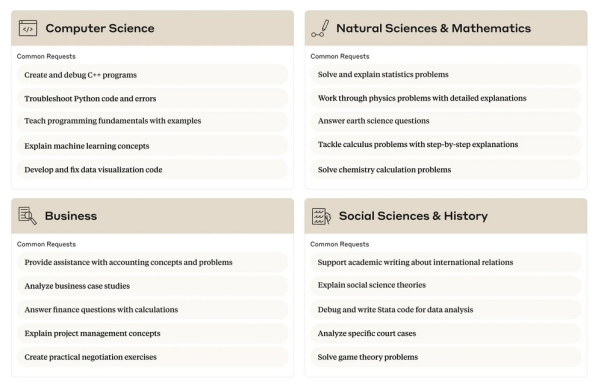
\includegraphics[keepaspectratio]{index_files/mediabag/images/script01-01.pdf}}

}

\caption{\label{fig-script}Wofür Studierende LLMs nutzen \emph{Quelle:}
Handa et al. (2025)}

\end{figure}%

\begin{figure}

\centering{

\pandocbounded{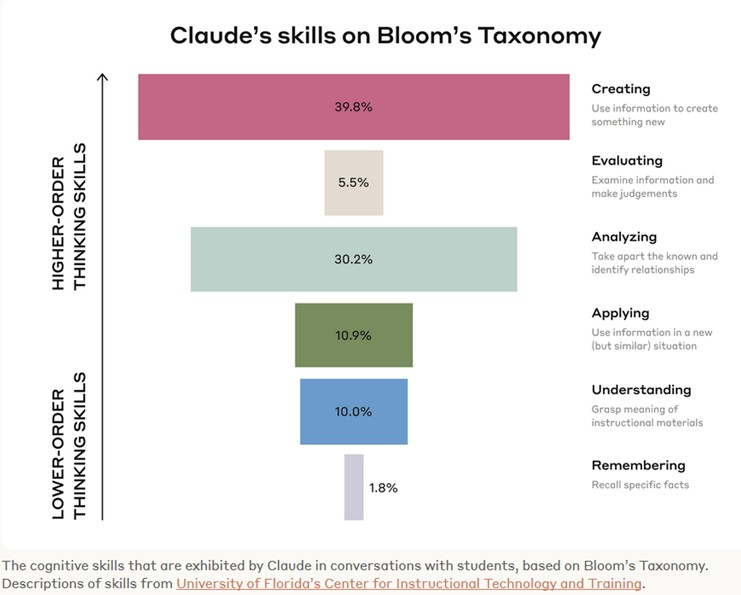
\includegraphics[keepaspectratio]{index_files/mediabag/images/script01-02.pdf}}

}

\caption{\label{fig-bloom-taxonomie}Schwerpunkte der Nutzung von LLMs
(Claude) durch Studierende nach der Bloom'schen Taxonomie. Quelle: Handa
et al. (2025)}

\end{figure}%

\textbf{Auch außerhalb der Hochschule steigt die Nutzung}. Eine Reihe
von Studien zeigen \textbf{erhöhte Produktivität von Büroarbeitenden mit
LLM-Unterstützung}: der Kundensupport arbeitet 15\% schneller, wenn das
Sprachmodell Antwortoptionen vorschlägt und Verweise auf interne
technische Dokumentation anbietet (Brynjolfsson et al., 2025),
Programmierer programmieren schneller (Peng et al., 2023), Consultants
sind produktiver bei komplexen Beratungsprojekten (Dell'Acqua et al.,
2023) und Sprachmodelle wie ChatGPT können eine Vielzahl kleiner
Aufgaben beschleunigen (Handa et al., 2025) und werden insofern gerade
zur Texterstellung schon millionenfach als Hilfsmittel im Beruf genutzt:
Von Kundenbewertungen über Pressemitteilungen und Stellenanzeigen (Liang
et al., 2025).

Die zunehmende Verwendung von KI in der Lehre hat gute Gründe. Wie oft
eine neue Technologie genutzt wird, hängt nach dem \textbf{Technology
Acceptance Model} (TAM) von der \textbf{wahrgenommenen
Benutzerfreundlichkeit} (perceived ease of use) und der
\textbf{wahrgenommenen Nützlichkeit} (perceived usefulness) ab
(\textbf{marangunić2015b?}). Generative KI wie ChatGPT decken sichtlich
beide Aspekte ab: Sie sind einfach zu nutzen (Kestin et al., 2025; Lee
et al., 2025; Monib et al., 2025; Naddaf, 2025b) und erzeugen einen
deutlichen Mehrwert, wie Studierende und Lehrende in einer Vielzahl von
Umfragen der letzten zwei Jahren berichten (Heidt, 2025; Morgan, 2024;
Ou et al., 2024). Lehrende ziehen nach: Meta-Untersuchungen zeigen ein
extremes Wachstum an Publikationen zur Nutzung von LLM im
Hochschulalltag (Ma, 2025; Ogunleye et al., 2024).

\section{Risiken und Nebenwirkungen}\label{risiken-und-nebenwirkungen}

Die Metapher mit dem E-Bike trägt allerdings auch, was die
\textbf{Risiken und Nebenwirkungen} angeht: Ab wann lässt die
maschinelle Unterstützung wichtige Muskeln verkümmern? Solche Gefahren
bestehen -- wie empirische Studien zeigen, erfordern die neuen Workflows
der Wissensarbeit durch KI-Unterstützung auch neue Formen der kritischen
Auseinandersetzung mit den Inhalten. Die Analyse von 1 Millionen
anonymisierten Studierenden-Chats durch Anthropic (Handa et al., 2025)
zeigt einerseits, dass \textbf{Studierende das LLM vor allem für
kognitiv anspruchsvollere Aufgaben einsetzen}, vor allem in den
Kategorien „Creating'' und „Analyzing'' (s.
Abbildung~\ref{fig-bloom-taxonomie}). Dies steht im deutlichen Gegensatz
zur Nutzung von einfachen Internetsuchen, die einen Schwerpunkt auf dem
Finden einzelner Fakten haben.

Wie kann man verhindern, dass die Studierenden kritische kognitive
Aufgaben allein den KI-Systemen übergeben? Eine Studie von 319
Wissensarbeitern zeigt, dass sich das \textbf{Gewicht zwischen den
Einzelaufgaben der Wissensarbeit mit LLMs verschiebt}: Der Aufwand für
die Recherchen selbst sinkt, es steigt anderseits der Aufwand für
Management-ähnliche Aufgaben: Koordination der Einzelaufgaben für Mensch
und Maschine, kritische Prüfung der berichteten Ergebnisse und die
Integration von Ergebnissen in den Gesamtprozess (etwa zur Erstellung
eines Gesamtberichtes, einer Test-Spezifikation oder eines Protokolls)
(Lee et al., 2025). Werden solche neuen Vorgehensweisen nicht geübt,
droht ein Rückgang des kritischen Denkens. Lehre heißt in diesem Kontext
auch, empfohlene Arbeitsweisen mit der neuen Technik zu üben.

\section{Kapitelübersicht}\label{kapiteluxfcbersicht}

Im Folgenden werden wir zunächst einige \textbf{Grundbegriffe} klären:
Was sind große Sprachmodelle und was ist mit Begriffen wie Token, Prompt
und RAG gemeint? \textbf{Welche Modelle} können Lehrende aktuell nutzen
und welche \textbf{Empfehlungen für Prompts} sind belastbar (Abschnitt
2.5)? Dann fragen wir nach \textbf{Zielen}: Welche Art von Wissen und
Methoden unterscheidet und empfiehlt die Lernforschung? Welche
\textbf{didaktischen Wirkmechanismen} können durch KI genutzt werden, um
typische Probleme der Hochschullehre anzugehen (Abschnitt 3)? Im
Abschnitt 4 schauen wir auf \textbf{Praxisbeispiele} für vier
Anwendungsfelder von Sprachmodellen an Hochschulen: \textbf{KI als Hiwi}
(direkte Arbeitserleichterung), \textbf{KI als Copilot} (Unterstützung
beim Schreiben und Coden) und \textbf{KI als Tutor} (Feedback und
Lernunterstützung) sowie \textbf{KI als Simulator} (Role Play und Goal
Play). Abschließend zeigen wir verschiedene Anwendungen von KI in
verschiedenen Kurstypen und gehen auf neue \textbf{Herausforderungen für
Prüfungen} ein (Abschnitt 5). Im Appendix werden Risiken von KI,
rechtliche Rahmenbedingungen und konkrete Prompts und Aufgabenbeispiele
aufgeführt.

\bookmarksetup{startatroot}

\chapter{Grundbegriffe}\label{grundbegriffe}

\section{Definition einiger
Grundbegriffe}\label{definition-einiger-grundbegriffe}

Hier führen wir kurz ein, was es mit Begriffen wie Transformer, Token,
Kontextfenstern und Prompts auf sich hat. Technische Details klammern
wir dabei aus, es geht nur um eine kurze Begriffsbestimmung.

Als visuelle Begleitung empfehle ich das sehr schöne Einführungsvideo
des Mathematik-Didaktikers Grant Sanderson (7 Minuten). Tiefer in die
mathematischen Details geht die grafische und interaktive Einführung als
Animation von Brendan Bycroft. Wer tiefer in die Hintergründe einsteigen
will, kann das Lehrbuch-Standardwerk von Jurafsky \& Martin (2025)
nutzen, das online frei verfügbar ist.

\begin{tcolorbox}[enhanced jigsaw, titlerule=0mm, left=2mm, title=\textcolor{quarto-callout-tip-color}{\faLightbulb}\hspace{0.5em}{Lernspiel: Begriffe prüfen}, leftrule=.75mm, colframe=quarto-callout-tip-color-frame, colback=white, rightrule=.15mm, breakable, opacityback=0, bottomtitle=1mm, toprule=.15mm, colbacktitle=quarto-callout-tip-color!10!white, toptitle=1mm, arc=.35mm, bottomrule=.15mm, coltitle=black, opacitybacktitle=0.6]

Wollen Sie gleich prüfen, welche der Begriffe Sie schon kennen?

Hier ist ein kleines \textbf{Lernspiel} (als Artifact mit dem
Sprachmodell Claude erstellt), in dem Sie die Begriffe den richtigen
Definitionen zuordnen müssen:
\href{https://claude.site/artifacts/d8e3cee4-ea47-48e3-a84c-a774d408aac8}{\ul{https://claude.site/artifacts/d8e3cee4-ea47-48e3-a84c-a774d408aac8}}

(am besten auf dem Computer spielen).

\end{tcolorbox}

Ein \textbf{Large Language Model (LLM)} ist ein fortschrittliches
maschinelles Lernmodell, das speziell darauf trainiert ist, menschliche
Sprache zu verstehen und Texte zu erzeugen, die natürlich erscheinen.
Die Modelle können erstaunliche Mengen von Textdaten verarbeiten, um
vielseitige Sprachanwendungen zu ermöglichen.

Die \textbf{generative Künstliche Intelligenz} (GenAI) bezieht sich auf
Systeme, die fähig sind, neue Inhalte zu erzeugen, wie etwa Texte, die
noch nicht existierten. LLMs sind ein zentraler Teil dieser generativen
KI und können eigenständig Texte zu einem breiten Spektrum von Themen
generieren.

Das \textbf{Sprachmodell} (s. Abbildung 3) zerlegt dazu grob gesagt
Inputs wie Texte in kleine Bausteine (Tokens), verwandelt diese in
Zahlen (Embeddings), erkennt mithilfe komplexer Muster (Transformer und
Attention) deren Zusammenhänge, und erzeugt auf diese Weise
selbstständig basierend auf kontextbezogen berechneten
Wahrscheinlichkeiten neue Texte (generative Sprachproduktion).

\begin{figure}

\centering{

\pandocbounded{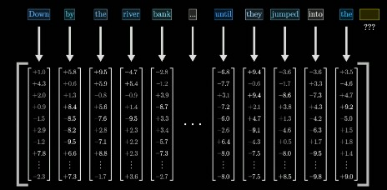
\includegraphics[keepaspectratio]{index_files/mediabag/images/script02-01.pdf}}

}

\caption{\label{fig-transformer}Visualisierung von
Transformator-Sprachmodellen. Quelle: Grant Sanderson,
https://youtu.be/LPZh9BOjkQs}

\end{figure}%

Sprachmodelle wie ChatGPT funktionieren insofern wie ein sehr gut
trainierter \textbf{Autovervollständiger} für Texte. Wenn man ihm den
Anfang eines Satzes gibt, sagt es mit hoher Wahrscheinlichkeit voraus,
wie der Satz weitergeht -- basierend auf Milliarden von Textbeispielen,
die es zuvor „gelesen`` hat.

Damit GPT Sprache verstehen und erzeugen kann, zerlegt es jeden Text in
sogenannte \textbf{Tokens} -- kleine Bausteine wie Wörter, Wortteile
oder Satzzeichen. Jedes dieser Tokens wird in einen \textbf{Vektor}
umgewandelt -- eine Zahlenreihe, die das Wort mathematisch beschreibt.
Dieser Vorgang nennt sich \textbf{Embedding}. Dabei wird darauf
geachtet, dass ähnliche Wörter ähnliche Vektoren erhalten,
beispielsweise „Hund`` und „Katze``.

Das Herzstück von GPT, dem Generative Pre-trained Transformer, ist der
sogenannte \textbf{Transformer} -- ein Rechenmodell, das durch ein
spezielles Aufmerksamkeitsverfahren (\textbf{Attention}) erkennt, welche
Wörter im Zusammenhang wichtig sind. Dadurch kann GPT die Bedeutung von
Wörtern im Kontext richtig einschätzen. GPT „achtet`` besonders auf
bestimmte Tokens (Wörter oder Satzteile), die für die jeweilige Aussage
wichtig sind (s. @fig-transformer). Damit bestimmt das Modell, welche
Begriffe stärker zur Bedeutung beitragen und in welchem Verhältnis sie
zueinander stehen.

Beispielsweise erkennt GPT dank Attention in einem Satz wie „Die Bank
steht unter einem Baum`` anhand des Kontextes, ob „Bank`` ein Möbelstück
oder eine Institution meint. Attention ist ein zentraler Bestandteil des
Transformer-Modells und sorgt dafür, dass GPT Texte nicht nur wortweise,
sondern im Gesamtkontext verstehen und sinnvoll vervollständigen kann.

GPT wurde mit riesigen Textmengen \textbf{vortrainiert}
(\textbf{Pretraining}), ohne konkrete Aufgaben lösen zu müssen -- dieser
Vorgang erfolgt unüberwacht (\emph{unsupervised learning}).

Sprachmodelle nutzen häufig die Methode \textbf{„Reinforcement Learning
with Human Feedback`` (RLHF)}, um noch bessere Texte zu generieren.
Dabei erzeugt das LLM zunächst verschiedene Textversionen, die von
menschlichen Bewertern nach Qualität beurteilt werden. Diese Bewertungen
dienen dazu, das Modell zusätzlich zu trainieren und zu steuern, indem
Texte belohnt werden, die von Menschen als besonders gut, klar oder
hilfreich eingeschätzt wurden. Durch diesen Prozess „lernt`` das LLM,
Texte zu bevorzugen, die nicht nur sprachlich richtig, sondern für
Menschen besonders verständlich und nützlich sind.

Das macht es möglich, dass GPT später aus wenigen Stichworten neue Texte
generieren kann -- also kreativ Sprache produziert, ohne bloß zu
kopieren (generativ). Der Begriff „\textbf{generativ}`` bedeutet in
diesem Zusammenhang, dass GPT eigenständig neue, sinnvolle Texte
erzeugen kann, indem es gelernte Muster neu kombiniert, anstatt fertige
Texte zu übernehmen.

\textbf{Token} sind die Bausteine der Sprachverarbeitung in LLMs und
repräsentieren oft Wörter oder Satzzeichen. Die Zerlegung von Text in
Token ermöglicht es dem Modell, mit Sprache auf einer granularen Ebene
zu arbeiten. Auf Webseiten wie Tiktokenizer können wir selbst Text
eingeben und diese Zerlegung ausprobieren.

\begin{figure}

\centering{

\pandocbounded{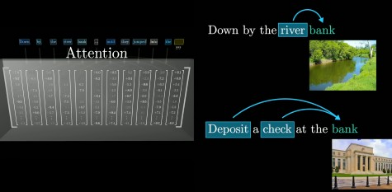
\includegraphics[keepaspectratio]{index_files/mediabag/images/script02-02.pdf}}

}

\caption{\label{fig-token}Beispiel für die Umwandlung von Text in Token}

\end{figure}%

\textbf{Was behält das Sprachmodell von unserer Unterhaltung? Wie viel
Text kann ich -- auch als PDF -- hochladen?} Neuere LLMs können schon
ganze Bücher schnell aufsaugen und dann zusammenfassen (z.B. Claude,
GPT-4o oder Gemini). Das \textbf{Kontext-Fenster} eines LLM beschreibt
die Menge an vorherigem Text, die das Modell bei der Verarbeitung neuer
Informationen berücksichtigt, um den Kontext und die Zusammenhänge zu
verstehen.

Ein \textbf{Prompt} ist eine Eingabeaufforderung, die an ein LLM
gesendet wird, um eine spezifische Antwort zu erhalten. Die Gestaltung
dieser Prompts ist entscheidend für die Qualität der generierten
Antworten und wird als \textbf{Prompt Engineering} bezeichnet.

\textbf{Agenten} im Kontext von KI sind fortgeschrittene Prompts, die
spezifische Aufgaben in natürlicher Sprache umsetzen. GPT-basierte
Agenten können Text analysieren, generieren und verschiedene Aufgaben
automatisieren, indem sie vorab definierte Muster und Regeln befolgen.
Durch die Erstellung solcher Agenten können Lehrende interaktive und
personalisierte Lerninhalte einfacher gestalten.

\textbf{RAG (Retrieval-Augmented Generation)} beschreibt die
Möglichkeit, zusätzliche Daten wie Fachtexte, Statistiken oder
Gesetzesbücher in Kombination mit einem KI Modell zu nutzen. Die KI ist
das Gehirn, die zusätzliche Wissensdatenbank quasi das Bücherregal, das
zu Rate gezogen werden kann. Je nach Kontextfenster stehen dort mehr
oder weniger Bücher. Insofern umschreibt RAG ein KI-Modell, das die
Fähigkeiten von Textgenerierungsmodellen (wie GPT) mit einer
Wissensdatenbank kombiniert. So wird etwa der Prompt-Agent (s.u.) mit
einer Reihe von Fachtexten „gefüttert``, in denen Best Practices des
Prompting erklärt werden.

Das Modell sucht nach relevanten Daten und integriert diese in die
generierte Antwort. In der Lehre kann RAG verwendet werden, um den
Studierenden Fachtexte oder besonders aktuelle Informationen zur
Verfügung zu stellen. Beispielsweise könnten Studierende in einem
Geschichtsseminar eine KI befragen, die externe Quellen durchforstet, um
aktuelle Erkenntnisse zu historischen Ereignissen zu präsentieren.
Unternehmen nutzen diese Technik, um etwa 1000-seitige
Gebrauchsanweisungen mit KI durchsuchbar zu machen, oder Chatbots zu
trainieren, die typische, repetitive Kundenanfragen beantworten.
Insofern ermöglicht RAG eine dynamische und zeitgemäße
Wissensvermittlung, die nicht auf das festgelegte Wissen des KI-Modells
beschränkt ist.

\section{Wie denken Sprachmodelle und warum halluzinieren
sie?}\label{wie-denken-sprachmodelle-und-warum-halluzinieren-sie}

Eine Studie des KI-Labors Anthropic hat mit neuen Methoden den
\textbf{Denkprozess eines Sprachmodells im Detail nachgezeichnet}
Lindsey et al. (2025), was uns erstmals etwas genauer verstehen lässt,
wie Sprachmodelle mit verschiedenen Sprachen umgehen, wie sie den
Schreibprozess „planen``, wie sie bei Kalkulationen vorgehen, wie weit
ihre Selbsterkenntnis reicht und warum sie manchmal Antworten erfinden
(„halluzinieren``).

\begin{figure}

\centering{

\pandocbounded{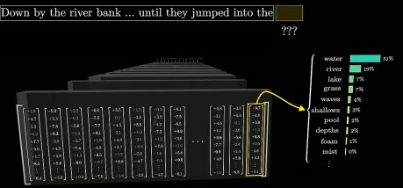
\includegraphics[keepaspectratio]{index_files/mediabag/images/script02-03.pdf}}

}

\caption{\label{fig-thoughtprocess}Visualisierte Gedanken eines
Sprachmodells {[}@lindsey2025a{]}}

\end{figure}%

\begin{itemize}
\tightlist
\item
  \textbf{Sprachübergreifend gleich:} Das Modell nutzt einen gemeinsamen
  sprachübergreifenden Bedeutungsraum.
\item
  \textbf{Textplanung:} Bei der Texterstellung plant das Modell mehrere
  Wörter im Voraus.
\item
  \textbf{Paralleles Rechnen:} Für Kalkulationen nutzt das Modell
  parallele Rechenpfade, die am Ende verbunden werden.
\item
  \textbf{Man traue nicht der Selbstkenntnis:} Das Modell erfindet
  manchmal Argumentationsketten (\emph{motivated reasoning}).
\item
  \textbf{Bekanntheit führt zu Halluzinationen:} Wenn das Modell eine
  genannte Entität „kennt`` (hier: den Namen des Forschers, Karpathy),
  aber nicht die Antwort auf die Frage (Titel des Fachartikels) führt
  das zu erfundenen Antworten (die „can't answer``-Funktion wird
  unterdrückt).
\end{itemize}

Claude nutzt einen \textbf{gemeinsamen Bedeutungsraum für verschiedene
Sprachen} -- ein Hinweis auf eine Art „universelle Denksprache``. Claude
verarbeitet Informationen in einem sprachunabhängigen, abstrakten
Bedeutungsraum. Bei der Frage nach dem „Gegenteil von klein`` in
verschiedenen Sprachen (z.\,B. Englisch, Französisch, Chinesisch)
aktivieren sich im Modell dieselben internen Merkmale für „Kleinheit``
und „Gegenteil``, unabhängig von der Eingabesprache. Erst in einem
späteren Schritt wird die Antwort in die jeweilige Zielsprache
übersetzt. Diese Erkenntnis legt nahe, dass Claude Wissen und Konzepte
sprachübergreifend anwenden kann.

\textbf{Plant das Sprachmodell die Textgeneration?} Entgegen der
Annahme, dass Sprachmodelle Texte strikt Wort für Wort basierend auf dem
unmittelbaren Kontext generieren, zeigt Claude die Fähigkeit, mehrere
Wörter im Voraus zu planen. In Aufgaben zur Gedichtgenerierung
identifiziert Claude beispielsweise Reimwörter, bevor es die
vorhergehenden Zeilen formuliert. Ein Beispiel: Soll ein Gedicht mit dem
Wort „Kaninchen`` enden, wählt Claude dieses Zielwort frühzeitig aus und
gestaltet die Zeile so, dass sie darauf hinführt. \hspace{0pt}Diese
Fähigkeit zur Vorausplanung deutet darauf hin, dass Claude in der Lage
ist, komplexe Textstrukturen zu erstellen, die über einfache
Wortassoziationen hinausgehen.

\textbf{Wie kalkulieren Sprachmodelle?} Anthropic hat in seiner Studie
zu Claude 3.5 Haiku detailliert untersucht, wie das Modell mathematische
Berechnungen intern verarbeitet. Dabei wurde festgestellt, dass Claude
bei Aufgaben wie der Addition von Zahlen parallele Rechenpfade nutzt, um
zu einem Ergebnis zu gelangen.\hspace{0pt} Claude verwendet zwei
Hauptpfade, um Additionen durchzuführen: 1. \textbf{Grobabschätzung:}
Ein Pfad schätzt das Ergebnis basierend auf den Größenordnungen der
Zahlen. 2. \textbf{Präzise Berechnung:} Ein anderer Pfad fokussiert sich
auf die genaue Berechnung, insbesondere auf die Bestimmung der letzten
Ziffer der Summe.

Diese beiden Pfade arbeiten zusammen, um das finale Ergebnis zu
erzeugen. Wenn beispielsweise der Pfad für die letzte Ziffer deaktiviert
wird, liefert Claude nur eine grobe Schätzung, ohne die genaue Endziffer
korrekt zu bestimmen.

\textbf{Können wir das Modell fragen, wie es zu einem Ergebnis gekommen
ist?} Eher nicht. Anthropics Studie zeigt, dass das Modell bei komplexen
Aufgaben manchmal überzeugende, aber erfundene Argumentationsketten
präsentiert. Bei einfachen Berechnungen, wie der Quadratwurzel von 0,64,
lassen sich klare interne Rechenschritte nachweisen. Bei schwierigeren
Aufgaben, etwa der Berechnung des Kosinus einer großen Zahl, gibt Claude
jedoch vor, Berechnungen durchgeführt zu haben, obwohl keine
entsprechenden internen Prozesse erkennbar sind. In solchen Fällen
konstruiert das Modell plausible, aber unbegründete Erklärungen -- ein
Verhalten, das als „motiviertes Denken`` bezeichnet wird. Diese
Fähigkeit, überzeugend zu argumentieren, ohne tatsächlich die zugrunde
liegende Logik zu befolgen, kann für Nutzer irreführend sein. Die von
Anthropic entwickelten Interpretationswerkzeuge ermöglichen es, solche
untreuen Denkprozesse zu identifizieren, indem sie die tatsächlichen
internen Abläufe des Modells sichtbar machen. Dies ist ein wichtiger
Schritt, um die Zuverlässigkeit und Transparenz von KI-Systemen zu
verbessern.

\textbf{Was kann zu Halluzinationen führen?} Wie wir im oben gezeigten
Beispiel sehen, ist den Antworten des Sprachmodells nicht immer zu
trauen. Das LLM verfügt über einen standardmäßig aktiven „Refusal
Circuit``, der das Modell dazu bringt, keine Antwort zu geben, wenn es
keine ausreichenden Informationen hat. Wenn eine bekannte Entität
erfasst wird, aktiviert sich ein konkurrierender „Known
Entity``-Mechanismus, der den Refusal Circuit hemmt und eine Antwort
ermöglicht. Problematisch wird es, wenn Claude einen Namen erkennt, aber
keine spezifischen Informationen dazu hat. In solchen Fällen kann der
„Known Entity``-Mechanismus fälschlicherweise den Refusal Circuit
unterdrücken, was zu einer Halluzination führt. Ein Beispiel: Bei der
Frage nach einem Fachartikel des bekannten Forschers Karpathy gibt
Claude einen erfundenen Titel an, da das Modell zwar den Namen kennt, in
diesem Fall aber keine Informationen über den Artikel hat. Bei weniger
bekannten Namen gibt das Modell an, die Antwort nicht zu kennen Lindsey
et al. (2025).

\section{Welches Modell wählen?}\label{welches-modell-wuxe4hlen}

\textbf{Was für LLMs gibt es aktuell?} Die großen Anbieter mit den
jeweils stärksten Modellen (s. @fig-leaderboard) sind OpenAI (Chat
GPT-5), Google (Gemini 2.5) und Anthropic (Claude Opus 4.1 / Sonnet 4).
Je nach Anwendung werden günstigere Modelle angeboten, die weniger
Rechenaufwand benötigen, meist mit dem Zusatz „Mini``. Starke Reasoning
Modelle (die komplexe Fragestellungen bearbeiten können) von OpenAI sind
GPT 5 oder Gemini 2.5 Flash (Stand 08/2025). Kostenfrei nutzbare Open
Source Alternativen sind z.B. Mistral (eines der wenigen europäischen
Modelle) und Llama4 (von Meta/Facebook) sowie die chinesische Konkurrenz
DeepSeek V3.1 Ethan Mollick (2025a); sowie (\textbf{Vellum.ai?}).

\textbf{Welches Sprachmodell sollte man aktuell nutzen?} Die kurze
Antwort ist, dass aktuell \textbf{GPT-5 eine gute Wahl} ist. \textbf{Für
Lehrende kostenfrei nutzbar} gibt es aktuell (August 2025) den zentralen
Dienst „Chat-AI`` / Academic Cloud der Gesellschaft für
wissenschaftliche Datenverarbeitung Göttingen (GWDG)
(https://chat-ai.academiccloud.de/), über den neben einer Reihe von
quelloffenen Modellen mittlerweile auch Chat GPT-5 nutzbar ist. Hier
kann man sich einfach mit einer Hochschuladresse registrieren und den
Dienst nutzen. Hochschulen bieten teils einen eigenen KI-Zugang an, die
TH-Köln etwa einen begrenzten Zugang zu ChatGPT und einzelnen
quelloffenen Modellen über das THKI-Lab
(https://ki.th-koeln.de/login.php). \textbf{Ab dem 15.9. soll} an der TH
Köln und weiteren NRW-Hochschulen die Lösung KI:connect ausgerollt
werden, die ähnliche Funktionalitäten bereitstellt
(https://kiconnect.pages.rwth-aachen.de/pages/).

Außerdem können Lehrende über die Hochschullizenz Microsoft 365 Copilot
herunterladen und dann einen KI-Chat als Desktop-Anwendung nutzen, eine
Anwendung, unter deren Haube auch wieder verschiedene Versionen von
ChatGPT stecken (hier einloggen und einfach herunterladen:
https://www.office.com/). Hier kann man auch GPT 5 nutzen, Chats
speichern und komplexere Anweisungen als „Agenten`` entwerfen und
teilen.

Diese kostenfreien Lösungen sind in den letzten Monaten stark ausgebaut
worden und mittlerweile schon sehr nützlich geworden. Sie stellen
allerdings i.d.R. nicht den aktuellen Stand der Performanz der
KI-Modelle dar. Lehrende sollten daher unbedingt 1 bis 2 Monate die 20
Euro investieren und auch die stärksten Bezahlmodelle ausprobieren (also
ChatGPT oder Gemini in der Bezahlversion). Nur so erhält man ein Gefühl
dafür, was aktuell technisch möglich ist und wie „sicher`` die eigenen
Prüfungsleistungen sind (z.B. „im Gespräch`` mit der KI, über das Voice
Modell, was bei den kostenfreien Zugängen aktuell meist abgeklemmt ist).

\begin{figure}

\centering{

\pandocbounded{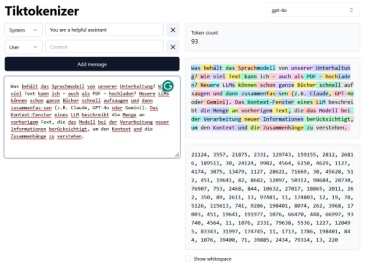
\includegraphics[keepaspectratio]{index_files/mediabag/images/script02-04.pdf}}

}

\caption{\label{fig-leaderboard}Je nach Ziel ein anderer Platz in der
Bestenliste: „Schlauste`` und günstigste Modelle. Quelle: Vellum.ai,
Stand 08/2025}

\end{figure}%

\textbf{Hier kann man vergleichen:} In der LM-Arena kann man
verschiedene Modelle ausprobieren und ihre Antwort auf eine bestimmte
Frage gegenüberstellen: https://lmarena.ai/ (Untermenü: „Arena
(side-by-side)``).

\section{Was können die Modelle -- und was
nicht?}\label{was-kuxf6nnen-die-modelle-und-was-nicht}

Was für Aufgaben LLMs beherrschen ist sehr uneinheitlich und
\textbf{verändert sich dynamisch}. Es gibt Bereiche, in denen heutige KI
auf menschlichem Niveau oder besser agiert, und andere, oft nur
geringfügig andersartige Aufgaben, an denen die KI (noch) scheitert
Dell'Acqua et al. (2023). Mollick und Kollegen prägen hierfür den
Begriff einer „\textbf{Jagged Technological Frontier}`` (zerklüftete
Technik-Grenze) Dell'Acqua et al. (2023). Zwei Aufgaben von ähnlicher
Schwierigkeit für Menschen können mit sehr unterschiedlicher Qualität
durch ein LLM gelöst werden -- eine liegt innerhalb der KI-Frontier
(d.~h. die KI kann sie lösen), die andere außerhalb (KI liefert
unbrauchbare oder falsche Resultate) Dell'Acqua et al. (2023).

In einem Experiment mit Consultants wurden 18 verschiedene
Beratungsaufgaben gestellt. Für die meisten („inside the frontier``)
brachte KI enorme Vorteile, doch bei einer gezielt außerhalb der
Frontier gewählten Aufgabe schnitt die KI-Gruppe deutlich schlechter ab:
Hier waren die Consultants in der Gruppe mit KI 19 Prozentpunkte weniger
häufig korrekt als die ohne KI Dell'Acqua et al. (2023). Dieses Ergebnis
unterstreicht die \textbf{Gefahr, LLMs unkritisch auf Probleme
anzuwenden, die ihre aktuellen Fähigkeiten übersteigen} -- die Leistung
fällt dann hinter menschliches Niveau zurück. Praktisch bedeutet die
Jagged Frontier, dass Organisationen und Individuen lernen müssen, die
Grenze der KI-Fähigkeiten zu erkennen und entsprechend zu navigieren
Dell'Acqua et al. (2023).

Für folgende Anwendungsfälle sind LLMs mittlerweile gut nutzbar Handa et
al. (2025); Korinek (2024-12 (update)); Schwarcz et al. (2025):

\begin{itemize}
\tightlist
\item
  Zusammenfassung von Fachartikeln
\item
  Fortgeschrittene mathematische Ableitungen
\item
  Anspruchsvolle Codierungsaufgaben
\item
  Erstellen eines Podcasts zu einer Forschungsarbeit
\item
  Erstellen von Präsentationsfolien
\item
  Verfassen von Blogbeiträgen
\item
  Simulieren von Interviews mit der Sprachausgabe von ChatGPT oder
  Gemini
\item
  KI-gestützte Suche (mit kritischer Prüfung natürlich)
\end{itemize}

Die Fähigkeiten der Modelle wuchsen in den letzten Monaten rasant und
damit werden die Aufgaben, die man an sie delegieren kann komplexer. Die
Länge der Aufgaben, die KI Sprachmodelle relativ genau erledigen können,
verdoppelt sich seit 2019 etwa alle 7 Monate Kwa et al. (2025). Auch die
Bewertung von Forschungsarbeiten im Rahmen des Peer-Reviews wird
zunehmend teil-automatisiert, etwa durch die automatische Prüfung von
Quellen oder Code und Teilbewertungen durch Dienste wie Veracity oder
Paper Wizard Lovely (2025); Naddaf (2025b).

\textbf{Ist das ein Mensch, oder ein Bot?} Eine neuere Studie zeigt,
dass neue Sprachmodelle uns bei dieser Frage mittlerweile
\textbf{erfolgreich täuschen können} und so den Turing Test bestehen, da
sie in einer sozialen Interaktion Menschen erfolgreich imitieren können
Jones \& Bergen (2025). In einem randomisierten
Drei-Parteien-Turing-Test mit über 1.000 Spielen wurde ein mit
speziellen Eingabe-Anweisungen (Persona-Prompt) versehenes Sprachmodell
(GPT-4.5) von den Respondenten zu 73 \% für den Menschen gehalten,
häufiger als echte Menschen in der Vergleichsgruppe. Weniger komplexe
Modelle (wie Llama 3.1) schritten schlechter ab. Die Autoren diskutieren
daraus resultierende Risiken von sozialer Manipulation oder
Arbeitsplatzsubstitution, sowie die Notwendigkeit robusterer
menschlicher Erkennungsstrategien.

Auch durch diesen Fähigkeitsschub ist der \textbf{Einsatz von
Sprachmodellen in Support-Funktionen wie Call Centern stark gestiegen},
empirische Studien belegen hier einen starken Produktivitätszuwachs
Brynjolfsson et al. (2025).

Die Gründe für die Produktivitätssteigerung von KI-Modellen lassen sich
durch \textbf{Scaling Laws} (Training Scaling Law, Inference Scaling
Law, Ethan Mollick (2025c), S. 3) beschreiben: KI-Modelle werden
einerseits exponentiell besser, je mehr Daten, Rechenleistung und
Parameter genutzt werden und andererseits, wenn sie mehr Zeit zum
„nachdenken`` erhalten.

Der erste Zusammenhang (\textbf{Training Scaling Law}) besagt, dass
größere KI-Modelle mit mehr Parametern und Trainingsdaten systematisch
leistungsfähiger werden\hspace{0pt}. Allerdings sind solche
Ertragszuwächse mit hohen Kosten verbunden: Eine 10-fache Steigerung an
Rechenaufwand führt etwa zu einer Erhöhung der Leistungsmetriken um
einen festen Betrag, was abnehmende Grenzerträge andeutet.

Neben dem positiven Effekt der Modellgröße wurde in den letzten Monaten
ein zweiter Scaling-Effekt (\textbf{Inference Scaling Law}) auf der
Anwenderseite deutlich: LLMs liefern bessere Lösungen, wenn man ihnen
mehr „\textbf{Denkzeit}`` gibt. OpenAI fand heraus, dass ein Modell mit
längerer Schritt-für-Schritt-Reasoning-Phase merklich bessere Ergebnisse
erzielt, analog zu einem Menschen, dem man mehr Zeit für eine schwierige
Aufgabe gibt. Dieser Inference Scaling Law führte zur Entwicklung von
\textbf{Reasonern} -- KI-Systemen, die bei Bedarf intern zusätzliche
Rechenschritte durchführen, um schwierige Probleme genauer zu lösen
Gottweis et al. (2025); OpenAI (2024); Schwarcz et al. (2025).

Zusammengenommen bedeuten diese Skalierungsgesetze, dass KI-Systeme
\textbf{durch höheren Ressourceneinsatz (beim Training und bei der
Nutzung) immer leistungsfähiger} und vielseitiger werden, wenn auch zu
steigenden Kosten. Ökonomisch relevant ist hier vor allem, dass die
\textbf{Grenzkosten der KI-Nutzung sehr niedrig} bleiben, sobald ein
großes Modell einmal trainiert ist: Ist das Modell erstellt, kann es
millionenfach eingesetzt werden, was \textbf{Skaleneffekte in der
Verbreitung} ermöglicht. Somit schafft das Scaling Law die Grundlage
dafür, dass \textbf{hochleistungsfähige KI als allgemein verfügbares
Gut} in Wirtschaft und Bildung eingesetzt werden kann. Durch diese
Eigenschaft ermöglicht KI eine schnelle und kosteneffiziente Skalierung
personalisierter und adaptiver Lernangebote E. R. Mollick \& Mollick
(2024). Dieses exponentielle Wachstum unterscheidet KI grundlegend von
bisherigen technologischen Entwicklungen, bei denen Verbesserungen oft
linear verliefen.

OpenAI hat allein in den ersten Monaten von \textbf{2025 mehrere neue
Funktionen} eingeführt, die den Einsatz von KI in der Hochschullehre
deutlich erweitern könnten: Mit der Bildgenerierungsfunktion in GPT4o
lassen sich nun auch fotorealistische Visualisierungen erstellen, was
z.B. in der technischen Bildung oder bei Designprojekten didaktisch
genutzt werden kann (März 2025). Die neuen Audio-Modelle ermöglichen
eine präzise Steuerung von Sprachstil und Tonfall -- hilfreich etwa für
simulierte Rollenspiele, interaktive Lernbegleiter oder barrierefreie
Lerninhalte (März 2025). Das im Februar eingeführte \textbf{deep
research}-Modul erlaubt KI-gestützte Rechercheprozesse, die Studierende
bei komplexen Projektarbeiten oder der Literatursichtung unterstützen
könnten (Februar 2025). Zusätzlich wurde mit \textbf{o3-mini} ein
kostengünstigeres Modell vorgestellt, das den Zugang zu leistungsfähigen
KI-Anwendungen auch in Bildungseinrichtungen erleichtert (Januar 2025).

\pandocbounded{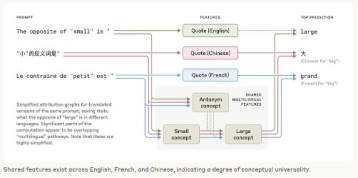
\includegraphics[keepaspectratio]{index_files/mediabag/images/script02-05.pdf}}.
Quelle: Lovely (2025), basierend auf Kwa et al. (2025)

Es lassen sich nach dieser Studie \textbf{zwei Kooperationsmodelle
zwischen Mensch und LLM} unterscheiden, um die Technologiegrenze optimal
auszunutzen Dell'Acqua et al. (2023): Der \textbf{Centaur-Ansatz} teilt
die Aufgabe, indem der Mensch der KI die Teilprobleme überlässt, die
innerhalb der Frontier liegen, und sich selbst auf den Rest
konzentriert. Der \textbf{Cyborg-Ansatz} integriert die KI tiefer, indem
der Mensch kontinuierlich mit der KI interagiert und Feedback-Schleifen
nutzt. Beide setzen implizit voraus, dass der Nutzer um die Stärken und
Schwächen des LLM weiß.

Eine spätere Studie des weitgehend selben Teams mit 776 Praktikern bei
Procter \& Gamble zeigt, dass Individuen mit LLM Unterstützung deutlich
produktiver Probleme lösen oder neue Ideen generieren konnten. Das
Sprachmodell scheint einen deutlichen Mehrwert als „\textbf{Cybernetic
Teammate}`` zu bringen und Einzelne teils auf das Leistungsniveau von
ganzen Teams zu bringen Dell'Acqua et al. (2025).

Wenn man \textbf{ältere oder weniger starke (offene) Modelle nutzt,
fährt man mit dem Fahrrad auf der Autobahn}. Vergleiche zeigen starke
Performanzunterschiede zwischen GPT-3.5 und den folgenden Updates zu
GPT-4 und GPT-4o. Auch die frei verfügbaren Modelle wie Llama sind teils
deutlich weniger „schlau``! Hier muss man insofern aufpassen, dass die
einfache Verfügbarkeit solcher Modelle über Plattformen wie Academic
Cloud nicht zu einem falschen Bild führt.

\section{Wo und wie spreche ich mit der
KI?}\label{wo-und-wie-spreche-ich-mit-der-ki}

\subsection{Wo sprechen? Verschiedene Zugänge zu
Sprachmodellen}\label{wo-sprechen-verschiedene-zuguxe4nge-zu-sprachmodellen}

\textbf{Wo} sprechen wir mit dem Sprachmodell? Welche Zugänge zur KI
gibt es? Es gibt \textbf{grob gesagt drei Ansätze}:

\begin{enumerate}
\def\labelenumi{\arabic{enumi}.}
\item
  Die einfache Eingabe in das Chat-Interface (z.B. bei Chat GPT oder
  Claude), ist am leichtesten umzusetzen. Um verschiedene Modelle zu
  nutzen, muss man sich aber neu einloggen und evtl. ein weiteres
  Abonnement bezahlen. Die meisten Modelle erlauben aber auch recht
  umfangreiche kostenlose Nutzung, was meist zum Kennenlernen ausreicht.
  Für Hochschulen werden zentral nach und nach verschiedene Dienste mit
  solchen Oberflächen aufgesetzt, die meist aber aus Gründen des
  Datenschutzes einige Funktionen abklemmen (z.B. meist die direkte
  Sprachinteraktion und das Speichern von Benutzerprofilen).
\item
  Nutzung einer Bedienoberfläche wie Witsy oder Typingmind, die Prompts
  speichert und Agenten erstellen lässt, die mit verschiedenen Modellen
  funktionieren Schwarze (2025). Hier muss man einmalig das System
  aufsetzen (Witsy) und für den höheren Komfort teils eine eine Lizenz
  kaufen (TypingMind, ca. 40 \$ für Hochschulangehörige), dafür kann man
  dann einfacher Modelle wechseln und über einen sogenannten API Key nur
  die tatsächliche Nutzung abrechnen (was sich bei einfacher Nutzung auf
  ein paar Cent beläuft, siehe die oben gezeigte Übersicht der Preise
  pro Millionen Token).
\item
  Wenn man sich nicht vor etwas Code scheut, kann man auch einfach
  selbst programmieren (mit KI-Unterstützung in Tools wie Google Colab)
  und kleine Sprachagenten aufsetzen. (Evtl. dann in Verbindung mit
  \textbf{Replit} für die Online-Bereitstellung und Diensten wie
  \textbf{Voiceflow} für die Oberfläche.) Auch hierfür braucht man
  eigentlich nur API Keys zur Identifizierung. Fragen Sie Chat GPT, wie
  das geht und lassen sich den Code schreiben, es ist überraschend
  einfach! Es gibt bei Youtube auch eine Vielzahl von kurzen
  Erläuterungen.
\end{enumerate}

\subsection{Wie sprechen?
Prompt-Befehle}\label{wie-sprechen-prompt-befehle}

\textbf{Wie} spreche ich mit dem LLM? Vorab die vielleicht wichtigste,
wenn auch banale Empfehlung: Es hilft, \textbf{genau zu sagen, was man
eigentlich will}. Man sollte nicht auf den Hiwi schimpfen, wenn man sich
nicht die Zeit genommen hat, zu sagen, was eigentlich die Aufgabe ist!

Wie beschreibe ich genau, was ich will? Einfache \textbf{Daumenregeln
für Prompts} gliedern das in vier Schritte: dem Sprachmodell eine
\textbf{Rolle} zuzuweisen („Du bist Verhandlungsexpertin``), ein klares
\textbf{Ziel} zu definieren („Du hilfst mir dabei, mich auf
Geschäftsverhandlungen vorzubereiten``), es zu bitten, sein
\textbf{Vorgehen} (den Gedankengang / „chain of thought``) offenzulegen
und Schritt-für-Schritt vorzugehen („Erstelle zunächst einen Plan und
frag mich nach Feedback. Warte meine Antwort ab und passe den Plan
eventuell an. Wenn ich zufrieden bin, beginne mit dem ersten Schritt in
deinem Plan.``) sowie \textbf{Beispiele} („few shot``) für eine
gewünschte Struktur oder Analyse mitzuliefern („Formatiere die
Dateinamen in dieser Form {[}Autor{]}-{[}Jahr{]}-{[}Kurztitel{]}``, oder
„Gib mir 5 Handlungsoptionen und nenne jeweils Vor- und Nachteile``).

Dabei veranlasst die Chain of Thought-Methode das LLM, seine
Gedankengänge offen zu legen. Das Modell zeigt seine Überlegungen
Schritt für Schritt, was die Nachvollziehbarkeit seiner Antworten
verbessert. So können wir auch besser nachsteuern und das Ergebnis an
unsere Ziele anpassen.

\begin{tcolorbox}[enhanced jigsaw, titlerule=0mm, left=2mm, title=\textcolor{quarto-callout-note-color}{\faInfo}\hspace{0.5em}{Hinweis}, leftrule=.75mm, colframe=quarto-callout-note-color-frame, colback=white, rightrule=.15mm, breakable, opacityback=0, bottomtitle=1mm, toprule=.15mm, colbacktitle=quarto-callout-note-color!10!white, toptitle=1mm, arc=.35mm, bottomrule=.15mm, coltitle=black, opacitybacktitle=0.6]

Wollen Sie sich interaktiv einen ausführlichen Prompt erstellen lassen?
Nutzen Sie diesen \textbf{Prompt-Bot}, den wir für Sie auf Basis der
Best-Practice Empfehlungen von OpenAI, Anthropic und wissenschaftlichen
Studien zu Prompt-Strategien erstellt haben:
\url{https://chatgpt.com/g/g-sF6vTgq2U-prompt-bot}

\end{tcolorbox}

Neuere empirische Untersuchungen haben eine Reihe von
\textbf{anekdotischen Hausrezepten des Promptings systematisch geprüft
und meist widerlegt}. Prompts funktionieren nicht immer gleich und so
kommt es schnell zu anektodischer Evidenz, dass eine Formulierung
„besser geklappt`` hätte. Die wenigsten der Empfehlungen helfen
zuverlässig Meincke et al. (2025b); Meincke et al. (2025a); Meincke et
al. (2025c){]}. Hilft es, \textbf{höflich} zu sein (nein), zu
\textbf{drohen} (nein), \textbf{Geld} anzubieten (nein), oder den
Hiwi-Bot \textbf{Schritt für Schritt} vorgehen zu lassen (ja, aber das
machen die neueren Reasoning-Sprachmodelle auch selbst)?

Für die Lehre wollen wir \textbf{den Prompts speziell didaktische
Elemente hinzufügen}, also etwa verhindern, dass den Studierenden sofort
eine Lösung ausgegeben wird, da das eigene Nachdenken in Form von Fragen
und sokratischem Dialog ihnen dabei hilft, die Ergebnisse auch zu
behalten Roediger \& Pyc (2012). Konkrete und sehr detaillierte
\textbf{Prompt-Beispiele speziell für die Lehre} finden Sie im Appendix
3: Ausgewählte Prompts zur Lehr- und Lernunterstützung. Weitere
Beispiele dafür finden sich in der Prompt-Bibliothek von Ethan Mollick
(https://www.moreusefulthings.com/prompts).

Gerade \textbf{für „Agenten``}, die einigermaßen zuverlässig bestimmte
Aufgaben erfüllen sollen, lohnt es sich aber im Sinne der o.g.
Empfehlung (sag, was Du willst), sehr detaillierte Prompts mit
Beispielen zu formulieren. Wer hier tiefer einsteigen will, kann hier
die \textbf{detaillierten Empfehlungen der KI-Labore zum Prompt-Design
lesen:} von Anthropic/Claude, alternativ hier die Details von OpenAI.

\section{Wie steht es mit dem Energieverbrauch der
Modelle?}\label{wie-steht-es-mit-dem-energieverbrauch-der-modelle}

Durch das starke Wachstum der neuen Technologie, werden wir verstärkt
mit den möglichen Effekten von KI auf Ressourcenverbrauch und
Umweltbelastung konfrontiert Spencer \& Singh (2025). Auch bei der
Nutzung in der Lehre wird dies regelmäßig von Studierenden angesprochen.
In diesem Bereich gibt es viel Hype und Desinformation in beide
Richtungen (von „Weltuntergang durch KI-Energiehunger!{}`` zu „keinerlei
Problem``), so dass hier ein kurzer Überblick seriöser Studien nützlich
erscheint. Dieser sehr knappe Abriss soll vor allem eine kurze
Orientierung und den Verweis auf weiterführende Literatur zur vertieften
Beschäftigung bieten.

\textbf{Wie schmutzig ist es also, KI zu nutzen? Die kurze Antwort} ist,
dass ein typischer Prompt aktuell etwa soviel Energie verbraucht wie ca.
10 Sekunden Netflix-Streaming oder eine typische Google Suche im Jahre
2008 Elsworth et al. (2025); Ethan Mollick (2025c). Die gute Nachricht
ist, dass die Modelle effizienter werden und der Energieverbrauch pro
Output-Token rasant sinkt und dass die Anreize für die großen Anbieter
stark darauf ausgerichtet sind, den Energieverbrauch weiter zu senken.
Gegenläufig und problematisch ist die stark steigende Nutzung, die z.B.
zur Ausweitung gerade umweltbelastender Energieformen wie Gasturbinen
führt Wittenberg (2025).

\textbf{Solche Vergleiche sind nicht trivial}, da etwa bei der Nutzung
in Unternehmen auch die Umweltfolgen der aktuellen Alternativen
„bepreist`` werden müssen, um einen sinnvollen Vergleich zu erzielen.
Wie belastet die Lieferkette eines physischen Buchs die Umwelt im
Vergleich zu einem E-Book? Ein aktueller Mitarbeiter im physischen
Callcenter mit seinem Arbeitsweg, Schreibtisch und Heizbedarf im
Vergleich zum KI-Chatbot? Unabhängig davon, wie diese Rechnungen
ausgehen, sind sie sichtlich komplex.

Im Folgenden sollen dazu einige Kernaussagen aus Untersuchungen der
International Energy Agency (IEA), dem World Economic Forum und des MIT
Technology Reviews zusammengefasst werden. Basierend auf die aktuelle
Untersuchung des MIT Technology Survey O'Donnell \& Crownhart (2025)
gliedere ich diesen kurzen Abriss zum Energieverbrauch in vier Teile:
Die Modellbildung, die Anfrage (query), die Emissionen und Prognosen für
das weitere Wachstum.

\textbf{Modellbildung.} Daten-Zentren und KI-Nutzung machen aktuell nur
wenige Prozent der globalen Energienutzung aus. Schätzungen der
Energieagentur IEA liegen etwa bei 3-5\%. Deutlich höhere Anteile liegen
in den Bereichen Gebäude, Industrie und Fahrzeuge Ritchie (2024a);
Spencer \& Singh (2024). Mit Blick auf die Zukunft ist der rasant
wachsende Energiebedarf durch Bevölkerungswachstum und wachsenden
Wohlstand ärmerer Bevölkerungsgruppen bei weitem ein stärkerer Treiber
für Emissionswachstum und Klimawandel Spencer \& Singh (2024). Einige
Klimaaktivisten warnen sogar vor „distraction`` - davor, sich durch
solche Ablenkungen und Modethemen wie KI Energieverbrauch von dem Fokus
auf die großen Hebel der Emissionsvermeidung ablenken zu lassen Masley
(2025); Ritchie (2024b). Während die Einmalaufwände für das Training der
Modelle erheblich sind, hat das schnelle Wachsen der Nutzerzahlen sie
mittlerweile in den Schatten gestellt. Die Energieaufwände für Anfragen
(Inferenz) bedingen nunmehr einen größeren Energieverbrauch als das
Training der Modelle O'Donnell \& Crownhart (2025); Spencer \& Singh
(2025).

\textbf{Anfrage.} Der Energieverbrauch einer einzelnen KI-Textanfrage
ist relativ gering. Er liegt unter dem Energieverbrauch von wenigen
Minuten für eine kleine LED-Lampe. Konkret liegen die Schätzungen hier
aktuell zwischen 0.3 Wattstunden (Wh) für GPT-4o und 0.03 Wh für kleine
Modelle O'Donnell \& Crownhart (2025); You (2025){]}.

\textbf{Im Vergleich zu anderen Energieverbrauchen ist das nicht viel.}
Vergleicht man den höheren Wert von 0.3 Wh mit den 12.000 Wattstunden,
die ein durchschnittlicher britischen Haushalt pro Tag verbraucht (für
US-Haushalte wird die deutlich höhere Zahl von 28.000 Wattstunden pro
Tag genannt!), wird schnell klar, dass weniger KI-Nutzung zumindest
aktuell kein großer Hebel für Energiesparen oder Klimaschutz ist. Die
oft zitierte Statistik, nach der eine Anfrage bei ChatGPT 10x mehr
verbraucht als eine Google Suche vergisst meist zu erwähnen, dass die
Basisrate dieser Internetnutzung im Vergleich zu anderen Dingen, in die
unser Energieverbrauch fließt, extrem niedrig ist Ritchie (2024b).

\textbf{Modellgröße ist allerdings ein zentraler Faktor für den
Energiebedarf} pro Anfrage und hieraus speisen sich plausiblere Sorgen.
Zwar ist Bildgenerierung i.d.R. weniger energieintensiv als
Textgenerierung, da Modelle zur Bildgenerierung oft mit weniger
Parametern arbeiten als Textmodelle. Aber komplexere Anfragen (etwa
mehrstufige lange Reasoning Aufträge) und speziell Video-Generierung
benötigen deutlich mehr Energie: Ein hochqualitatives Video von 5
Sekunden kann bis zu 1.000 Wattstunden verbrauchen (0.94 kWh), was etwas
mehr als einer Stunde Mikrowellennutzung entspricht -- ein deutlicher
Unterschied O'Donnell \& Crownhart (2025).

\textbf{Der Anteil größerer Modelle und komplexerer Anfragen wird
voraussichtlich deutlich zunehmen}, wenn die Modellgrößen weiter
ansteigen und komplexere Anfragen, wie Video-Generierung zunehmen.
Gegenläufig wirkt der starke Anreiz für die Anbieter (und speziell für
die kleineren Konkurrenten von OpenAI, die über geringere finanzielle
Mittel verfügen), den Energieverbrauch pro Inferenz durch effizientere
Chip-Konstruktionen und neue Trainingsansätze zu senken. Wie die
Analysten der IEA zusammenfassen: „The efficiency of AI-related computer
chips has doubled roughly every two-and-a-half to three years, and a
modern AI-related computer chip uses 99\% less power to perform the same
calculations as a model from 2008'' Spencer \& Singh (2024).

Insgesamt wird perspektivisch die punktuelle Einzelnutzung durch
\textbf{einzelne Anfragen weniger wichtig werden, als die strukturell
bedingte Integration der KI-Technologien} in immer mehr digitale
Anwendungen, die als Folge des rasanten technologischen Wandels und der
hohen Investitionen absehbar ist O'Donnell \& Crownhart (2025).

\textbf{Emissionen.} In diesem Zusammenhang wird der ungünstige
Energiemix der aktuell entstehenden Datenzentren kritisiert: Da
KI-Rechenzentren rund um die Uhr laufen und meist in Regionen mit
fossilen Energieträgern stehen, ist der durchschnittliche CO₂-Ausstoß
ihrer Stromversorgung etwa 48\,\% höher als der US-Durchschnitt
O'Donnell \& Crownhart (2025). Dem gegenüber stehen \textbf{gegenläufige
Effekte wie höhere Effizienz der Steuerung}, etwa von Energienetzen
Greene-Dewasmes \& Tladi (2025) und dem \textbf{Ersatz von manuellen
menschlichen Aufwänden durch Digitalisierung}, etwa durch Reisen für
einen Film-Dreh (ohne KI) oder dem Energiebedarf eines menschlichen
Call-Centers. Das starke Wachstum der Nutzung muss insofern mit
politischer Anreizsetzung für emissionslose Energiegewinnung verbunden
sein, wenn eine starke Zunahme an Emissionen vermieden werden soll.
Hierfür gibt etwa die IEA klare Empfehlungen und technische Lösungen
sind bekannt. Besorgt stimmt die Analysten die Prognose eines starken
Wachstums von Datencentern im asiatischen Raum, die meist nicht mit
emissionsfreier Energie betrieben werden Spencer \& Singh (2025).

\textbf{Prognose.} In der Summe sehen viele der Untersuchungen
\textbf{Probleme eher in der prognostizierten zukünftigen Entwicklung
als in den aktuellen Energieaufwänden}. Das starke prognostizierte
Wachstum könnte etwa dazu führen, dass KI-Anwendungen bis 2028 mehr als
12\% des US-Strombedarfs ausmachen O'Donnell \& Crownhart (2025).

\section{Energieverbrauch und politische
Steuerung}\label{energieverbrauch-und-politische-steuerung}

Die \textbf{IEA} prognostiziert ebenfalls eine \textbf{Verdreifachung
des Energieverbrauchs von Rechenzentren bis 2030}, getrieben durch KI.
Maßnahmen wie \textbf{Effizienzgewinne} und \textbf{nachhaltige
Architektur} können diese Entwicklung abbremsen (Spencer \& Singh
(2025)).

Wie der \textbf{MIT-Bericht} hervorhebt, sollte vor diesem Hintergrund
der starke und kurzfristig induzierte Ausbau der Infrastruktur
\textbf{politisch durch Anreize zur Emissionsvermeidung gesteuert}
werden, sodass ein starkes Wachstum der Emissionen durch diesen --
wahrscheinlich im Kern unvermeidlichen -- technologischen Wandel
vermieden wird (O'Donnell \& Crownhart (2025)).

So besteht die Hoffnung, dass \textbf{positive Effekte auf Emissionen}
in den Hauptbereichen von CO₂-Emissionen (Gebäude, Industrie, Transport
sowie die verbundenen Energienetze) durch \textbf{höhere Effizienz in
Planung und Nutzung} genutzt werden können, ohne dass sie durch die
wachsenden Kosten von immer komplexeren Inferenz-Anfragen überlagert
werden (Greene-Dewasmes \& Tladi (2025); Spencer \& Singh (2025)).

Politisch gesehen ergibt sich insofern ein \textbf{Bedarf an Steuerung
dieses strukturellen technologischen Wandels}, damit die Ziele denen der
Gesellschaft entsprechen. Dazu müssen die \textbf{Fakten klar sein}: Um
Kosten und Effekte abschätzen, abfedern und verteilen zu können, fordern
die Forscher eine \textbf{deutlich höhere Transparenz der Energiebedarfe
durch die Modellanbieter} (O'Donnell \& Crownhart (2025)).

\bookmarksetup{startatroot}

\chapter{Ziele und didaktische
Mechanismen}\label{ziele-und-didaktische-mechanismen}

\section{Was für Ziele verfolgen wir mit dem Einsatz von GenAI in der
Lehre?}\label{was-fuxfcr-ziele-verfolgen-wir-mit-dem-einsatz-von-genai-in-der-lehre}

\bookmarksetup{startatroot}

\chapter{Vier Szenarien: Hiwi, Copilot, Tutor,
Simulator}\label{vier-szenarien-hiwi-copilot-tutor-simulator}

\section{Wie nutzen Lehrende aktuell generative
KI?}\label{wie-nutzen-lehrende-aktuell-generative-ki}

\bookmarksetup{startatroot}

\chapter{Empfehlungen zur Umsetzung}\label{empfehlungen-zur-umsetzung}

\section{Prompts anpassen,
experimentieren}\label{prompts-anpassen-experimentieren}

\section{Ausrichtung der Anpassungen nach Empfehlungen der
Lernforschung}\label{ausrichtung-der-anpassungen-nach-empfehlungen-der-lernforschung}

\section{Einführung der Studierenden planen: Besser praktisch, häufig
und
niedrigschwellig}\label{einfuxfchrung-der-studierenden-planen-besser-praktisch-huxe4ufig-und-niedrigschwellig}

\section{Wie prüfen wir jetzt? Jenseits der Homework
Apocalypse}\label{wie-pruxfcfen-wir-jetzt-jenseits-der-homework-apocalypse}

\section{Richtlinien zur KI-Nutzung - welche Handreichungen geben
Hochschulen}\label{richtlinien-zur-ki-nutzung---welche-handreichungen-geben-hochschulen}

\section{Beispiele für die Kurs-Integration von
KI}\label{beispiele-fuxfcr-die-kurs-integration-von-ki}

\section*{Wie bleiben Sie informiert?}\label{wie-bleiben-sie-informiert}
\addcontentsline{toc}{section}{Wie bleiben Sie informiert?}

\phantomsection\label{refs}
\begin{CSLReferences}{1}{0}
\bibitem[\citeproctext]{ref-brown2014a}
Brown, P. C., Roediger, H. L., \& McDaniel, M. A. (2014). \emph{Make it
stick: The science of successful learning}. Belknap Press.

\bibitem[\citeproctext]{ref-brown2014d}
Brown, P. C., Roediger III, H. L., \& McDaniel, M. A. (2014). \emph{Make
it stick: The science of successful learning}. Harvard University Press.

\bibitem[\citeproctext]{ref-brynjolfsson2025}
Brynjolfsson, E., Li, D., \& Raymond, L. (2025). Generative AI at work.
\emph{The Quarterly Journal of Economics}, qjae044.

\bibitem[\citeproctext]{ref-dellacqua2025b}
Dell'Acqua, F., Ayoubi, C., Lifshitz-Assaf, H., Sadun, R., Mollick, E.
R., Mollick, L., Han, Y., Goldman, J., Nair, H., Taub, S., \& Lakhani,
K. R. (2025). \emph{The Cybernetic Teammate: A Field Experiment on
Generative AI Reshaping Teamwork and Expertise}. Social Science Research
Network. \url{https://doi.org/10.2139/ssrn.5188231}.

\bibitem[\citeproctext]{ref-dellacqua2023a}
Dell'Acqua, F., McFowland, E., Mollick, E. R., Lifshitz-Assaf, H.,
Kellogg, K., Rajendran, S., Krayer, L., Candelon, F., \& Lakhani, K. R.
(2023). \emph{Navigating the Jagged Technological Frontier: Field
Experimental Evidence of the Effects of AI on Knowledge Worker
Productivity and Quality}. \url{https://doi.org/10.2139/ssrn.4573321}.

\bibitem[\citeproctext]{ref-elsworth2025a}
Elsworth, C., Huang, K., Patterson, D., Schneider, I., Sedivy, R.,
Goodman, S., Townsend, B., Ranganathan, P., Dean, J., \& Vahdat, A.
(2025). Measuring the environmental impact of delivering AI at Google
Scale. \emph{arXiv preprint arXiv:2508.15734}.

\bibitem[\citeproctext]{ref-gottweis2025a}
Gottweis, J., Weng, W.-H., Daryin, A., Tu, T., Palepu, A., Sirkovic, P.,
Myaskovsky, A., Weissenberger, F., Rong, K., Tanno, R., Saab, K.,
Popovici, D., Blum, J., Zhang, F., Chou, K., Hassidim, A., Gokturk, B.,
Vahdat, A., Kohli, P., \ldots{} Natarajan, V. (2025). \emph{Towards an
AI co-scientist}. arXiv.
\url{https://doi.org/10.48550/ARXIV.2502.18864}.

\bibitem[\citeproctext]{ref-greene-dewasmes2025a}
Greene-Dewasmes, G., \& Tladi, T. (2025, Januar 21). \emph{AI's energy
dilemma: Challenges, opportunities, and a path forward}.
\url{https://www.weforum.org/stories/2025/01/ai-energy-dilemma-challenges-opportunities-and-path-forward/}.

\bibitem[\citeproctext]{ref-handa2025c}
Handa, K., Tamkin, A., McCain, M., Huang, S., Durmus, E., Heck, S.,
Mueller, J., Hong, J., Ritchie, S., Belonax, T., Troy, K. K., Amodei,
D., Kaplan, J., Clark, J., \& Ganguli, D. (2025).
\emph{\href{https://assets.anthropic.com/m/2e23255f1e84ca97/original/Economic_Tasks_AI_Paper.pdf}{Which
economic tasks are performed with AI? Evidence from millions of claude
conversations}} (Report). Anthropic.

\bibitem[\citeproctext]{ref-hattie2023}
Hattie, J. (2023). \emph{Visible learning, the sequel: a synthesis of
over 2,100 meta-analyses relating to achievement}. Routledge, Taylor \&
Francis Group. \url{https://doi.org/10.4324/9781003380542}.

\bibitem[\citeproctext]{ref-heidt2025a}
Heidt, A. (2025). ChatGPT for students: learners find creative new uses
for chatbots. \emph{Nature}, \emph{639}(8053), 265--266.
\url{https://doi.org/10.1038/d41586-025-00621-2}.

\bibitem[\citeproctext]{ref-henderson2007a}
Henderson, C., \& Dancy, M. H. (2007). Barriers to the use of
research-based instructional strategies: The influence of both
individual and situational characteristics. \emph{Physical Review
Special Topics---Physics Education Research}, \emph{3}(2), 020102.

\bibitem[\citeproctext]{ref-invertedstone2025}
InvertedStone (2025, August 30). \emph{OpenAI API Pricing Calculator}.
\url{https://invertedstone.com/calculators/openai-pricing}.

\bibitem[\citeproctext]{ref-jones2025a}
Jones, C. R., \& Bergen, B. K. (2025). \emph{Large Language Models Pass
the Turing Test}. arXiv.
\url{https://doi.org/10.48550/arXiv.2503.23674}.

\bibitem[\citeproctext]{ref-jurafsky2025a}
Jurafsky, D., \& Martin, J. H. (2025).
\emph{\href{https://web.stanford.edu/~jurafsky/slp3/}{Speech and
language processing: An introduction to natural language processing,
computational linguistics, and speech recognition with language
models}}.

\bibitem[\citeproctext]{ref-kestin2025}
Kestin, G., Miller, K., Klales, A., Milbourne, T., \& Ponti, G. (2025).
AI tutoring outperforms in-class active learning: an RCT introducing a
novel research-based design in an authentic educational setting.
\emph{Scientific Reports}, \emph{15}(1), 17458.
\url{https://doi.org/10.1038/s41598-025-97652-6}.

\bibitem[\citeproctext]{ref-korinek2024b}
Korinek, A. (2024-12 (update)). LLMs Learn to Collaborate and Reason:
December 2024 Update to ``Generative AI for Economic Research: Use Cases
and Implications for Economists. \emph{Journal of Economic Literature},
\emph{61}(4), 1281--1317. \url{https://doi.org/10.1257/jel.20231736}.

\bibitem[\citeproctext]{ref-kwa2025a}
Kwa, T., West, B., Becker, J., Deng, A., Garcia, K., Hasin, M., Jawhar,
S., Kinniment, M., Rush, N., Arx, S. V., Bloom, R., Broadley, T., Du,
H., Goodrich, B., Jurkovic, N., Miles, L. H., Nix, S., Lin, T., Parikh,
N., \ldots{} Chan, L. (2025). \emph{Measuring AI Ability to Complete
Long Tasks}. arXiv. \url{https://doi.org/10.48550/arXiv.2503.14499}.

\bibitem[\citeproctext]{ref-lee2025a}
Lee, H.-P. H., Sarkar, A., Tankelevitch, L., Drosos, I., Rintel, S.,
Banks, R., \& Wilson, N. (2025). \emph{The Impact of Generative AI on
Critical Thinking: Self-Reported Reductions in Cognitive Effort and
Confidence Effects From a Survey of Knowledge Workers}.

\bibitem[\citeproctext]{ref-liang2025a}
Liang, W., Zhang, Y., Codreanu, M., Wang, J., Cao, H., \& Zou, J.
(2025). The Widespread Adoption of Large Language Model-Assisted Writing
Across Society. \emph{arXiv preprint arXiv:2502.09747}.

\bibitem[\citeproctext]{ref-lindsey2025a}
Lindsey, J., Gurnee, W., Ameisen, E., Chen, B., Pearce, A., Turner, N.
L., Citro, C., Abrahams, D., Carter, S., Hosmer, B., Marcus, J., Sklar,
M., Templeton, A., Bricken, T., McDougall, C., Cunningham, H., Henighan,
T., Jermyn, A., Jones, A., \ldots{} Batson, J. (2025).
\href{https://transformer-circuits.pub/2025/attribution-graphs/biology.html}{On
the biology of a large language model}. \emph{Transformer Circuits
Thread}.

\bibitem[\citeproctext]{ref-lovely2025a}
Lovely, G. (2025). AI could soon tackle projects that take humans weeks.
\emph{Nature}. \url{https://doi.org/10.1038/d41586-025-00831-8}.

\bibitem[\citeproctext]{ref-ma2025a}
Ma, T. (2025). Systematically visualizing ChatGPT used in higher
education: Publication trend, disciplinary domains, research themes,
adoption and acceptance. \emph{Computers and Education: Artificial
Intelligence}, \emph{8}, 100336.
\url{https://doi.org/10.1016/j.caeai.2024.100336}.

\bibitem[\citeproctext]{ref-masley2025a}
Masley, A. (2025, April 28). A cheat sheet for why using ChatGPT is not
bad for the environment.
\url{https://andymasley.substack.com/p/a-cheat-sheet-for-conversations-about}.

\bibitem[\citeproctext]{ref-mcafee2024}
McAfee, A. (2024).
\emph{\href{https://ide.mit.edu/wp-content/uploads/2024/04/Davos-Report-Draft-XFN-Copy-01112024-Print-Version.pdf?x76181}{Generally
Faster: The Economic Impact of Generative AI}} (Davos Report).
\textless{} bound method Organization. get\_name\_with\_acronym
of\textless{} Organization: Google~\ldots.

\bibitem[\citeproctext]{ref-meincke2024a}
Meincke, L., Mollick, E. R., \& Terwiesch, C. (2024). \emph{Prompting
Diverse Ideas: Increasing AI Idea Variance}.
\url{https://papers.ssrn.com/abstract=4708466}.

\bibitem[\citeproctext]{ref-meincke2025}
Meincke, L., Mollick, E., Mollick, L., \& Shapiro, D. (2025a).
\emph{Prompting Science Report 1: Prompt Engineering is Complicated and
Contingent}. arXiv. \url{https://doi.org/10.48550/arXiv.2503.04818}.

\bibitem[\citeproctext]{ref-meincke2025a}
Meincke, L., Mollick, E., Mollick, L., \& Shapiro, D. (2025b).
\emph{Prompting Science Report 2: The Decreasing Value of Chain of
Thought in Prompting}. arXiv.
\url{https://doi.org/10.48550/arXiv.2506.07142}.

\bibitem[\citeproctext]{ref-meincke2025c}
Meincke, L., Mollick, E., Mollick, L., \& Shapiro, D. (2025c).
\emph{Prompting Science Report 3: I'll pay you or I'll kill you -\/- but
will you care?} arXiv. \url{https://doi.org/10.48550/arXiv.2508.00614}.

\bibitem[\citeproctext]{ref-mollick2025}
Mollick, Ethan (2025a, Januar 26). \emph{A new generation of AIs: Claude
3.7 and Grok 3}.
\url{https://www.oneusefulthing.org/p/a-new-generation-of-ais-claude-37}.

\bibitem[\citeproctext]{ref-mollick2025a}
Mollick, Ethan (2025b, Juni 23). \emph{GPT-5: It Just Does Stuff}.
\url{https://www.oneusefulthing.org/p/gpt-5-it-just-does-stuff}.

\bibitem[\citeproctext]{ref-mollick2025d}
Mollick, Ethan (2025c, August 7). \emph{Mass Intelligence}.
\url{https://www.oneusefulthing.org/p/mass-intelligence}.

\bibitem[\citeproctext]{ref-mollick2024f}
Mollick, E. R., \& Mollick, L. (2024). \emph{Instructors as Innovators:
a Future-focused Approach to New AI Learning Opportunities, With
Prompts}. \url{https://doi.org/10.2139/ssrn.4802463}.

\bibitem[\citeproctext]{ref-mollick2023a}
Mollick, E., \& Mollick, L. (2023). Assigning AI: Seven approaches for
students, with prompts. \emph{arXiv}.
\url{https://doi.org/10.48550/arXiv.2306.10052}.

\bibitem[\citeproctext]{ref-monib2025a}
Monib, W. K., Qazi, A., \& Mahmud, M. M. (2025). Exploring learners'
experiences and perceptions of ChatGPT as a learning tool in higher
education. \emph{Education and Information Technologies}, \emph{30}(1),
917--939. \url{https://doi.org/10.1007/s10639-024-13065-4}.

\bibitem[\citeproctext]{ref-morgan2024a}
Morgan, G. (2024, Juli 11).
\href{https://onedtech.philhillaa.com/p/what-students-want-when-it-comes-to-ai}{What
Students Want When It Comes To AI - The Digital Education Council Global
AI Student Survey 2024}. \emph{On EdTech Newsletter}.

\bibitem[\citeproctext]{ref-naddaf2025}
Naddaf, M. (2025a). How are researchers using AI? Survey reveals pros
and cons for science. \emph{Nature}.
\url{https://doi.org/10.1038/d41586-025-00343-5}.

\bibitem[\citeproctext]{ref-naddaf2025c}
Naddaf, M. (2025b). AI is transforming peer review --- and many
scientists are worried. \emph{Nature}, \emph{639}(8056), 852--854.
\url{https://doi.org/10.1038/d41586-025-00894-7}.

\bibitem[\citeproctext]{ref-odonnell2025a}
O'Donnell, J., \& Crownhart, C. (2025, Mai 20).
\href{https://www.technologyreview.com/2025/05/20/1116327/ai-energy-usage-climate-footprint-big-tech/}{We
did the math on AI's energy footprint. Here's the story you haven't
heard.} \emph{MIT Technology Review}.

\bibitem[\citeproctext]{ref-ogunleye2024a}
Ogunleye, B., Zakariyyah, K. I., Ajao, O., Olayinka, O., \& Sharma, H.
(2024). A Systematic Review of Generative AI for Teaching and Learning
Practice. \emph{Education Sciences}, \emph{14}(6), 636.
\url{https://doi.org/10.3390/educsci14060636}.

\bibitem[\citeproctext]{ref-openai2024a}
OpenAI (2024).
\emph{\href{https://openai.com/index/learning-to-reason-with-llms/}{Learning
to reason with LLMs}}.

\bibitem[\citeproctext]{ref-openai2025b}
OpenAI (2025, August 28). \emph{Introducing GPT-5}.
\url{https://openai.com/index/introducing-gpt-5/}.

\bibitem[\citeproctext]{ref-ou2024a}
Ou, A. W., Stöhr, C., \& Malmström, H. (2024). Academic communication
with AI-powered language tools in higher education: From a post-humanist
perspective. \emph{System}, \emph{121}, 103225.
\url{https://doi.org/10.1016/j.system.2024.103225}.

\bibitem[\citeproctext]{ref-peng2023a}
Peng, S., Kalliamvakou, E., Cihon, P., \& Demirer, M. (2023). \emph{The
Impact of AI on Developer Productivity: Evidence from GitHub Copilot}.
arXiv. \url{https://doi.org/10.48550/arXiv.2302.06590}.

\bibitem[\citeproctext]{ref-ritchie2024}
Ritchie, H. (2024a, September 19). \emph{What's the impact of artificial
intelligence on energy demand?}
\url{https://www.sustainabilitybynumbers.com/p/ai-energy-demand}.

\bibitem[\citeproctext]{ref-ritchie2024a}
Ritchie, H. (2024b, November 18). \emph{What's the carbon footprint of
using ChatGPT?}
\url{https://www.sustainabilitybynumbers.com/p/carbon-footprint-chatgpt}.

\bibitem[\citeproctext]{ref-roediger2012b}
Roediger, H. L., \& Pyc, M. A. (2012). Inexpensive techniques to improve
education: Applying cognitive psychology to enhance educational
practice. \emph{Journal of Applied Research in Memory and Cognition},
\emph{1}(4), 242--248.
\url{https://doi.org/10.1016/j.jarmac.2012.09.002}.

\bibitem[\citeproctext]{ref-schmidt2005a}
Schmidt, B., \& Tippelt, R. (2005). Besser Lehren-Neues von der
Hochschuldidaktik?

\bibitem[\citeproctext]{ref-schwarcz2025a}
Schwarcz, D., Manning, S., Barry, P. J., Cleveland, D. R., Prescott, J.
J., \& Rich, B. (2025). \emph{AI-Powered Lawyering: AI Reasoning Models,
Retrieval Augmented Generation, and the Future of Legal Practice}.
\url{https://doi.org/10.2139/ssrn.5162111}.

\bibitem[\citeproctext]{ref-schwarze2025a}
Schwarze, M. (2025, Juli 16).
\href{https://www.faz.net/pro/digitalwirtschaft/prompt-der-woche/ki-assistent-witsy-kann-kostenlos-das-chatgpt-monatsabo-ersetzen-110586296.html}{KI-Assistent
Witsy kann kostenlos das ChatGPT-Monatsabo ersetzen}. \emph{Frankfurter
Allgemeine Zeitung (FAZ)}.

\bibitem[\citeproctext]{ref-spencer2024a}
Spencer, T., \& Singh, S. (2024, Oktober 18). What the data centre and
AI boom could mean for the energy sector -- Analysis.
\url{https://www.iea.org/commentaries/what-the-data-centre-and-ai-boom-could-mean-for-the-energy-sector}.

\bibitem[\citeproctext]{ref-spencer2025a}
Spencer, T., \& Singh, S. (2025).
\emph{\href{https://www.iea.org/reports/energy-and-ai}{Energy and AI}}
(World Energy Outlook Special Report). International Energy Agency.

\bibitem[\citeproctext]{ref-wittenberg2025a}
Wittenberg, A. (2025, Mai 6).
\href{https://www.politico.com/news/2025/05/06/elon-musk-xai-memphis-gas-turbines-air-pollution-permits-00317582}{{„How
come I can't breathe?``}: Musk's data company draws a backlash in
Memphis - POLITICO}. \emph{Politico}.

\bibitem[\citeproctext]{ref-you2025a}
You, J. (2025, Februar 7). How much energy does ChatGPT use? \emph{Epoch
AI}.
\url{https://epoch.ai/gradient-updates/how-much-energy-does-chatgpt-use}.

\end{CSLReferences}




\end{document}
